\documentclass[12pt]{article}
\usepackage{geometry} 
\geometry{margin=1in}
\geometry{a4paper} 


\usepackage{textcomp}
\usepackage{booktabs}
\usepackage{array}
\usepackage{paralist}
\usepackage{verbatim} 
\usepackage{subfigure}
\usepackage{graphicx,caption}
\usepackage{placeins}
\usepackage{lipsum}
\usepackage{xcolor}
\usepackage{dcolumn}
\usepackage{sectsty}
\allsectionsfont{\sffamily\mdseries\upshape}
\usepackage{gensymb,amsmath,mathtools,amssymb}
\usepackage{flafter}
%\usepackage{parskip}
\usepackage[utf8]{inputenc}
\usepackage[english]{babel}
\usepackage{tocbibind}
\usepackage[toc,page]{appendix}
\captionsetup{width=\linewidth}
\usepackage{bm}
\usepackage{url}

\usepackage{pdflscape}

\newcommand{\half}{\frac{1}{2}}


\graphicspath{{./figs/}}

\title{Initial Sizing of 2020 ICLR hybrid rocket}
\author{Devansh Agrawal}
%\date{} 


\begin{document}

\maketitle


\section{Introduction}

This document provides an overview of the sizing analysis and results for the 10k SRAD hybrid entry by Imperial College London Rocketry. 

This is a working document, and as more information is fed into the system, the parameters may be updated.

\section{Flight performance requirement}

The first challenge was to estimate the performance requirements of the hybrid rocket to able to attain the target altitude with some margin. A separate document details the analysis, but a summary is provided here. 

We assume the rocket follows a bang-off control scheme - the rocket thrusts at its main engine's max thrust, $F_{max}$~Newtons for $t_{burn}$~seconds and then coasts the remaining part of the journey. In this scenario, the final altitude of the rocket, $h_f = \hat h_f c^2/g$, is entirely dependent on four non-dimensional parameters\footnote{Assumes exponential atmosphere, constant drag coefficient, perfectly vertical flight}:


\begin{enumerate}
\item The thrust to initial weight ratio, $\hat F = (F_{max})/(m_0 g)$

\item A drag parameter defined as\footnote{Note: This parameter is like the drag to weight ratio (except it uses $c$ as the velocity and $m_0$ as the mass)}, $ x \equiv (\half \rho c^2 c_d A)/(m_0 g)$

\item Propellant mass fraction, $MR \equiv m_p/m_0$

\item Atmosphere parameter, $\hat \beta = \beta c^2/g$

\end{enumerate}

Plugging in suitable parameters, we find the required propellant mass fraction as a function of the thrust to weight ratio, as in figure~\ref{fig:PMF}. 

%\FloatBarrier
\begin{figure}[htbp]
   \centering
   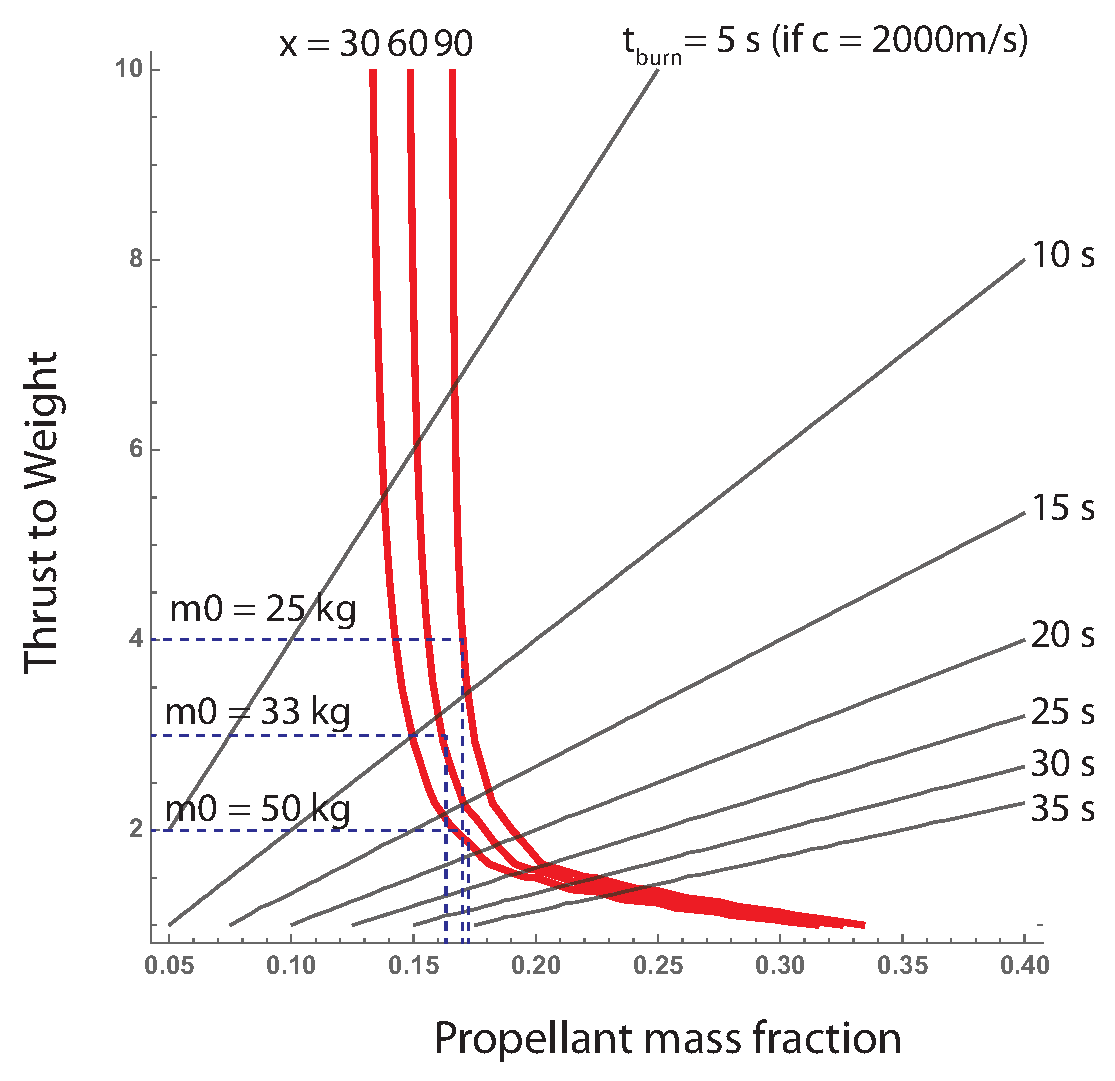
\includegraphics[width=0.8\linewidth]{perf_req.eps}
   \caption{Required thrust to weight ratio as a function of the propellant mass fraction}
   \label{fig:PMF}
\end{figure}
%FloatBarrier


From this, we can see that we need a propellant mass fraction of approximate 17\%. The fact that the lines are near vertical above $T/W>2$ suggests that a slow, low thrust burn is roughly equivalent to a fast, high thrust burn. Therefore, since we have the ability to control our burn during the flight, a long, slow burn allows us to turn off the thrust closer to apogee, and with greater certainty of success. 

\textbf{For design purposes, and to give ourselves some flexibility, we can therefore design our rocket to have a $T/W>2$ and a propellant mass fraction of at least 20\%. }

Detailed analysis with accurate drag coefficients, the mach dependence, and optimal control should be performed next to ensure these performance targets are sufficient and robust to future design changes. 

\section{Vehicle Architecture}

The chosen system breakdown of the rocket is:
 
\begin{enumerate}

\item Payload
\begin{itemize}
\item 4~kg payload
\item 4.5~kg allocated, to allow for mounting
\end{itemize}

\item Avionics
\begin{itemize}
\item Includes all flight computers and sensing equipment, switchboards and mounting hardware
\item Includes interface wiring to other components with electronics
\item Does not include mass of electronics for other subsystems
\item Allocated 2~kg, based on previous IREC reports.
\end{itemize}

\item Recovery System
\begin{itemize}
\item Includes main and drogue parachute, parachute lines and deployment mechanism mass
\item includes mass of black powder and associated electronics. 
\item Allocated 3~kg, based on previous IREC reports.
\end{itemize}

\item Main Engine
\begin{itemize}
\item Includes oxidiser tank, fuel tank
\item ox mass, fuel mass, 
\item valves assembly with electronics (allocated 1~kg), and nozzle assembly (allocated 1~kg)
\item Detailed engine sizing was not performed, and needs to be throughly verified. 
\end{itemize}

\item Boosters
\begin{itemize}
\item Since the $T/W$ of the main engine is around 2, it is not enough to clear the launch rail with the required speed. As such, solid boosters are to be used launch the rocket, sized to provide $T/W = 10$ for the duration needed to clear the launch rails.
\item Includes motor dry mass, but not mounting structural mass
\end{itemize}

\item Structures
\begin{itemize}
\item Includes nose cone (allocated 0.5 kg)
\item fins (1.2~kg)
\item body tube with internal bulkheads and couplers (4~kg)
\item booster mounting structure (0.3~kg)
\item overall structural mass allowed is 6~kg.
\end{itemize}

\end{enumerate}


\section{Sizing approach}

GPkit\footnote{\url{https://gpkit.readthedocs.io/en/latest/}} was used to perform the sizing study. GPkit allows the user to define variables describing the vehicle, the constraints relating the variables (either due to physics, performance requirements or due to design requirements), and an objective function to optimise. It will then perform a global optimisation and return the optimised parameters of the design. GPkit also allows for easy compartmentalisation, by allowing the user to define these variables within classes, and thus separating the different parts of the design. 

I have created a basic framework that should be general enough to allow more detail to be added into the model, as we develop it. 

At the top level, a \texttt{rocket} class is defined. The six components above are created, each defined in a separate python file. These classes inherit from \texttt{gpkit.Model} which allows gpkit to interpret the variables and the constraints, and exposes a \texttt{solve} method to perform the optimisation.

For ease of visualisation and interpretation, a jupyter notebook instantiates the \texttt{rocket} and calls the signomial solver, \texttt{localsolve}. Due to the structure of the rocket unfortunately, the geometric globally optimal solver cannot be called, but a local signomial solver must be used. That said, in most scenarios, this solver is sufficiently robust to return a good, and viable solution. 

The jupyter notebook also has result printing code blocks to allow for easy debugging of models. 

Note, when there are changes to the python files where the relationships are described, jupyter must re-import the classes. The best way to ensure this is accurately done is by clicking the \texttt{Restart \& Run-All} button. 

The most important relationships used in this sizing are listed at the end of the document, but the most up-to-date relationships are only available in the python files. 


\section{Sizing results}

The solve  took 5 GP solves, and 1.86 seconds. 

\textbf{Total rocket mass: 31.66~kg}

The results are more easily interpreted in the form of a diagram, on the last page.

\begin{landscape}

\begin{verbatim}
SORTED BY LINEAGE, SENSITIVITY (solved on 26-08 13:02)
+-------------------+---------------------+-----------+--------+--------+---------------------------------------+
|               key |             lineage |     value |   unit |   sens |                                 descr |
+-------------------+---------------------+-----------+--------+--------+---------------------------------------+
|               PMF |              Rocket |     0.200 |      - |  0.759 |     Propellant Mass Fraction required |
|        v_{launch} |              Rocket |    30.000 |    m/s |  0.107 |              Velocity off launch rail |
|        L_{launch} |              Rocket |     5.000 |      m | -0.014 |                 Length of launch rail |
|                 g |              Rocket |     9.810 |  m/s^2 |  0.010 |           Acceleration due to gravity |
|        a_{launch} |              Rocket |    90.000 |  m/s^2 |      * |          Acceleration off launch rail |
|                 m |              Rocket |    31.818 |     kg |      * |                        Mass of Rocket |
|    TW_{main, min} |              Rocket |     2.000 |      - |  0.000 | Main engine thrust to take off weight |
|             min_a |              Rocket |    90.000 |  m/s^2 |      * |           minimum launch acceleration |
|                 m |     Rocket/Avionics |     2.000 |     kg |  0.117 |                      Mass of Avionics |
|               DMF |     Rocket/Boosters |     0.700 |      - |  0.184 |         Dry mass fraction of boosters |
|                 c |     Rocket/Boosters |  2000.000 |    m/s | -0.079 |                boosters exhaust speed |
|                 m |     Rocket/Boosters |     1.348 |     kg |      * |                      Mass of Boosters |
|          m_{prop} |     Rocket/Boosters |     0.404 |     kg |      * |           Propellant mass of boosters |
|           m_{dry} |     Rocket/Boosters |     0.943 |     kg |      * |                  Dry mass of boosters |
|          t_{burn} |     Rocket/Boosters |     0.333 |      s |      * |                     Booster burn time |
|                 F |     Rocket/Boosters |  2425.711 |      N |      * |            Boosters cumulative thrust |
|                 m |      Rocket/Payload |     4.500 |     kg |  0.263 |                       Mass of Payload |
|                 m |     Rocket/Recovery |     3.000 |     kg |  0.176 |                      Mass of Recovery |
|      \sigma_{max} | Rocket/SimpleEngine |   430.000 |    MPa | -0.387 |        Max stress of tank, Al-7075-T6 |
|            Tank P | Rocket/SimpleEngine |    80.000 |    bar |  0.387 |                  Max Ox Tank pressure |
|                SF | Rocket/SimpleEngine |     5.000 |      - |  0.387 |          Wall thickness safety factor |
|    rho_{ox, tank} | Rocket/SimpleEngine |  2700.000 | kg/m^3 |  0.387 |            Density of ox tank (if al) |
|          rho_{ox} | Rocket/SimpleEngine |   490.000 | kg/m^3 | -0.327 |                  density of liquid ox |
|         rho_{wax} | Rocket/SimpleEngine |   900.000 | kg/m^3 | -0.059 |                       Density of fuel |
|        m_{valves} | Rocket/SimpleEngine |     1.000 |     kg |  0.059 |           Mass of valves and plumbing |
|        m_{nozzle} | Rocket/SimpleEngine |     1.000 |     kg |  0.059 |               Mass of nozzle assembly |
|                 F | Rocket/SimpleEngine |   750.000 |      N | -0.024 |                         Engine thrust |
|                OF | Rocket/SimpleEngine |     6.000 |      - | -0.004 |                      Ox to fuel ratio |
|              d_ox | Rocket/SimpleEngine |    15.000 |     cm |  0.000 |                   Diameter of ox tank |
|    m_{grain tank} | Rocket/SimpleEngine |     1.015 |     kg |      * |                    Mass of grain tank |
|                 m | Rocket/SimpleEngine |    14.970 |     kg |      * |                        Mass of Engine |
|       m_{ox tank} | Rocket/SimpleEngine |     5.592 |     kg |      * |                       Mass of ox tank |
|           m_{dry} | Rocket/SimpleEngine |     8.606 |     kg |      * |                    Dry mass of engine |
|          m_{prop} | Rocket/SimpleEngine |     6.364 |     kg |      * |                    Mass of Propellant |
|            m_{ox} | Rocket/SimpleEngine |     5.454 |     kg |      * |                               ox mass |
|          m_{fuel} | Rocket/SimpleEngine |     0.909 |     kg |      * |                             fuel mass |
|          t_{wall} | Rocket/SimpleEngine |     6.977 |     mm |      * |             Wall Thickness of ox tank |
|            V_{ox} | Rocket/SimpleEngine | 11131.502 |   cm^3 |      * |                     Volume of ox tank |
|            L_{ox} | Rocket/SimpleEngine |     0.630 |      m |      * |                     Length of ox tank |
|          v_{fuel} | Rocket/SimpleEngine |  1010.081 |   cm^3 |      * |                        Volume of fuel |
|         L_{grain} | Rocket/SimpleEngine |     0.114 |      m |      * |                   Length of the grain |
|         A_{grain} | Rocket/SimpleEngine |    88.312 |   cm^2 |      * |           cross section area of grain |
|          m_{tube} |   Rocket/Structures |     4.000 |     kg |  0.234 |                                  None |
|          m_{fins} |   Rocket/Structures |     1.200 |     kg |  0.070 |     Mass of fins and mounting of fins |
|            m_{nc} |   Rocket/Structures |     0.500 |     kg |  0.029 |                     Mass of nose cone |
| m_{booster_struc} |   Rocket/Structures |     0.300 |     kg |  0.018 |         Mass needed to mount boosters |
|                 m |   Rocket/Structures |     6.000 |     kg |      * |                    Mass of Structures |
+-------------------+---------------------+-----------+--------+--------+---------------------------------------+
\end{verbatim}

Note, the sensitivity is the logarithmic sensitivity, ie, $\text{sensitivity} = \frac{d \log(\text{cost})}{d\log(\text{var})}$. A positive number indicates that increasing the variable will increase the cost. Note, the star indicates a zero sensitivity, since this is a variable that gpkit has solved for. As such, it represents the minima of the function and thus has zero sensitivity, similar to how a function has zero gradient wrt to a variable when it is optimized. 

\end{landscape}


\section{Next steps}
\begin{itemize}
\item Verify structural mass allocations
\item Verify stability requirements - ie, ensure fins are large enough
\item Perform detailed drag accounting
\item Perform detailed controls analysis
\item more accurate tank sizing needed, especially considering manufacturability, source-ability, cost.
\item tank ullage not accounted for
\item very simplified thrust curve needs to be improved
\end{itemize}

Design modification if the engine performance is poorer than expected: bigger boosters. Therefore, the booster mounts need to be flexible enough to allow different booster designs. Could look into dropping boosters after their work is done, but this is complicated. 

%\bibliographystyle{unsrt}
%\bibliography{biblio}

\section{Sizing relationships used}

Most constraints are fairly straightforward. Here are the key ones

\begin{itemize}
\item m = sum of mass of components
\item propellant mass fraction $>$ 20\%
\item Launch requirements:
\begin{itemize}
\item v off launch rail $>$ 30m/s
\item launch accel = (booster thrust + main engine thrust - mg)/m 
\item launch accel $>$ min accel = (launch v)$^2$/(2 launch rail L)
\item booster burn time such that burn out occurs at 5 m/s
\end{itemize}
\item Components:
\begin{itemize}
\item Payload: m = 4.5 kg
\item Avionics: m = 2 kg
\item Recovery: m = 3 kg
\item Engine: 
\begin{itemize}
\item OF = 6
\item m fuel, m ox based on m prop and OF
\item d = 150 mm
\item P tank $<$ 80 bar
\item wall thickness based on hoop stress and safety factor of 5, assumes Al-7075 due to high yield strength (double of Al 6061), sealing and welding to be determined more thoroughly
\item ox is fully liquid, at critical density of 490 kg/m3 $\rightarrow$ determine length of ox tank
\item mass of ox tank based on cylinder material thickness, end caps not accounted for
\item grain tank is similarly sized, assumes the grain is only occupied in half the cross sectional area (needs to be refined), and same wall thickness as ox tank. No liner material considered. Carbon overwrap of tank tube would save lots of mass if possible. 
\item \emph{regression rates, motor dynamics, etc not accounted for}
\item m valves = 1 kg
\item m nozzle = 1 kg
\item assumed F= 750 N
\item c = 2100 m/s (needs to be verified)
\end{itemize}
\item Boosters:
\begin{itemize}
\item propellant mass such that total impulse can be delivered
\item dry mass fraction is 70\%. Needs to be refined by picking a motor, assumed c = 2000m/s
\end{itemize}
\item Structures:
\begin{itemize}
\item m = sum of components
\item m fins = 1.2 kg
\item m nose cone = 0.5 kg
\item m tube = 4 kg
\item m  booster struc = 0.3 kg
\end{itemize}
\end{itemize}

\end{itemize}


\FloatBarrier
\begin{figure}[htbp]
   \centering
   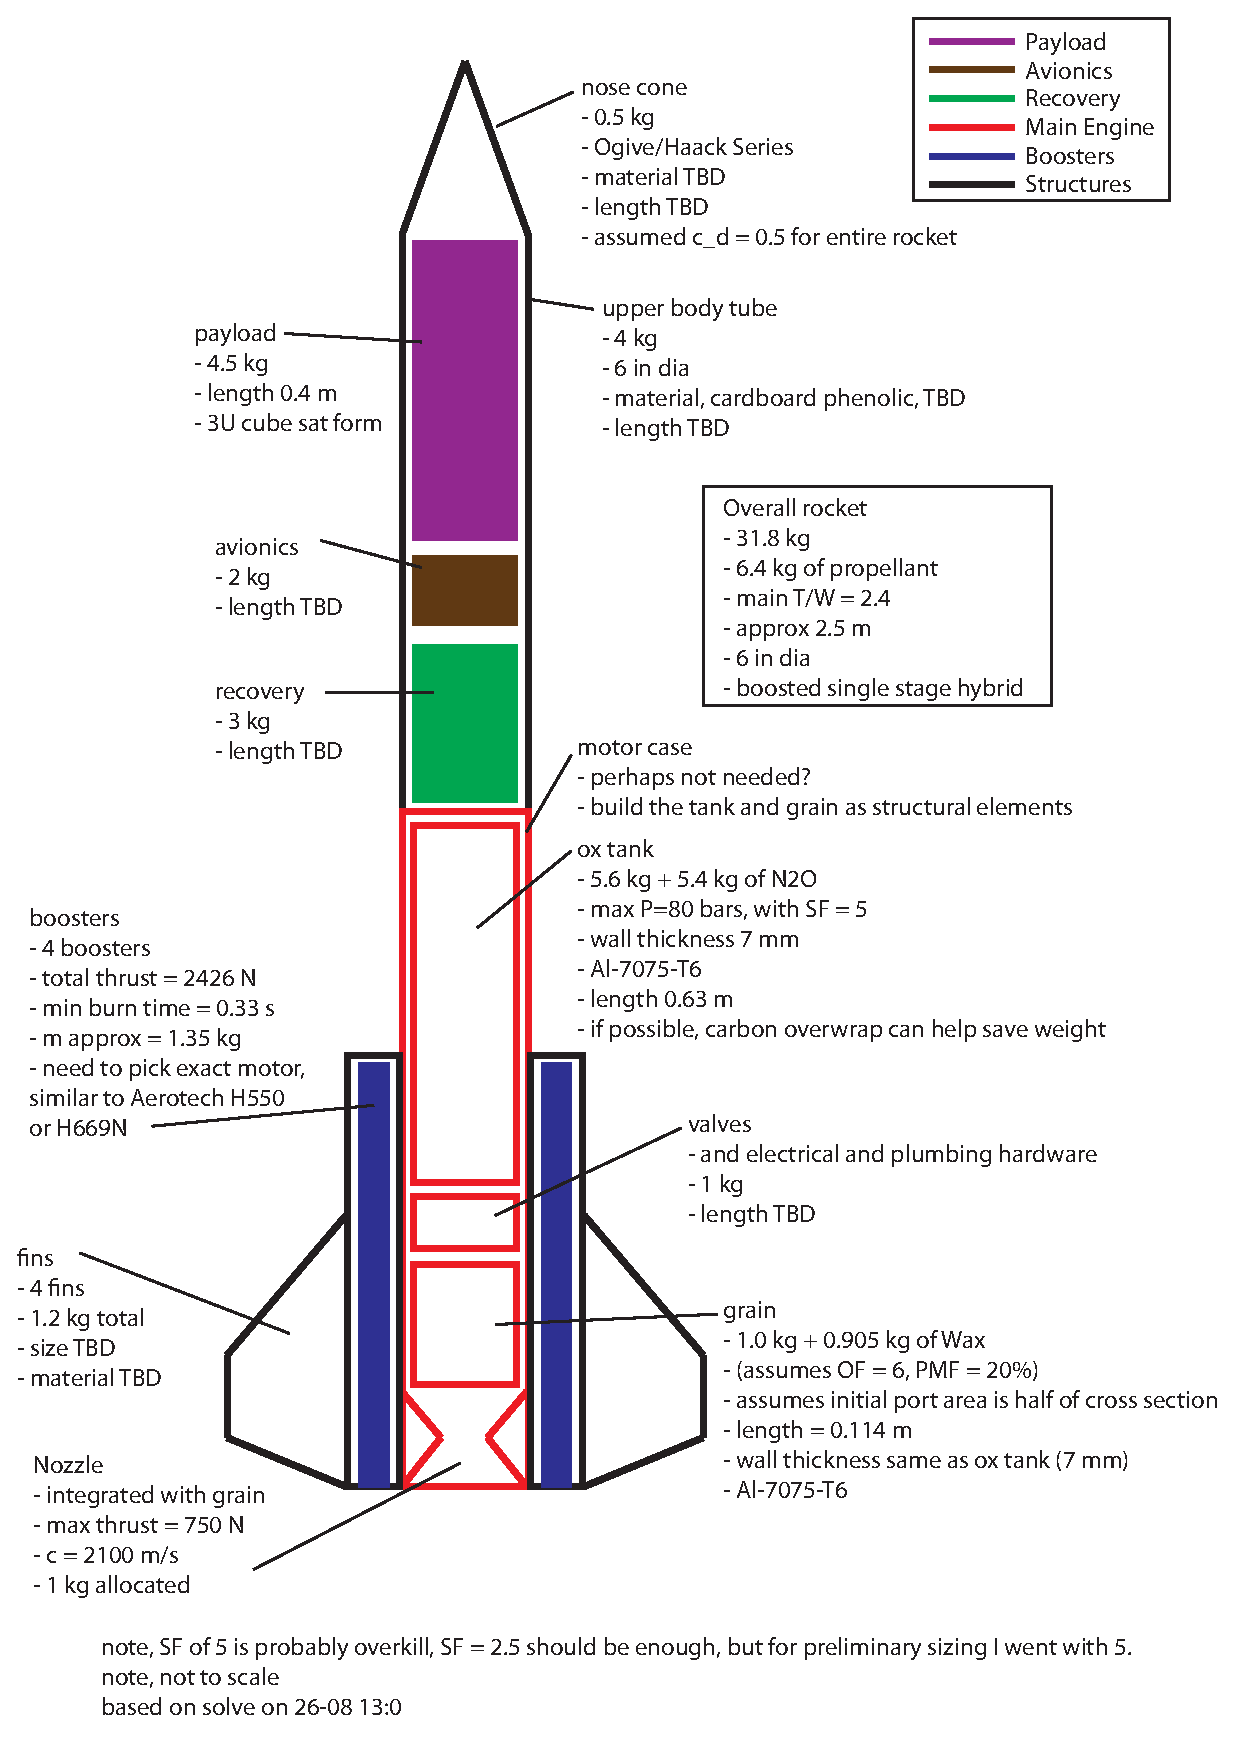
\includegraphics[width=\linewidth]{sizing_result_Aug_26.eps}
   \caption{Summary of Sizing results}
   \label{fig:}
\end{figure}
%FloatBarrier



\end{document}























